\documentclass{oblivoir}
\usepackage{amsmath,amssymb,amsthm,kotex,paralist,kswrapfig}

\usepackage[skipabove=10pt]{mdframed}

\usepackage{tabto,pifont}
\TabPositions{0.2\textwidth,0.4\textwidth,0.6\textwidth,0.8\textwidth}
\newcommand\tabb[5]{\par\noindent
\ding{172}{#1}
\tab\ding{173}{#2}
\tab\ding{174}{#3}
\tab\ding{175}{#4}
\tab\ding{176}{#5}}

\usepackage{enumitem}
%\setlist{noitemsep}
\setlist[enumerate]{label=(\arabic*)}

\newcounter{num}
\newcommand{\defi}[1]
{\bigskip\noindent\refstepcounter{num}\textbf{정의 \arabic{num}) #1}\par\noindent}
\newcommand{\theo}[1]
{\bigskip\noindent\refstepcounter{num}\textbf{정리 \arabic{num}) #1}\par\noindent}
\newcommand{\exam}[1]
{\bigskip\noindent\refstepcounter{num}\textbf{예시 \arabic{num}) #1}\par\noindent}
\newcommand{\prob}[1]
{\bigskip\noindent\refstepcounter{num}\textbf{문제 \arabic{num}) #1}\par\noindent}
\newcommand{\proo}
{\bigskip\textsf{증명)}\par}

\newcommand{\ans}{
{\par
\raggedleft\textbf{답 : (\qquad\qquad\qquad\qquad\qquad\qquad)}
\par}\bigskip\bigskip}

\newcommand{\pb}[1]%\Phantom + fBox
{\fbox{\phantom{\ensuremath{#1}}}}

\newcommand\ov[2]{\ensuremath{\overline{#1#2}}}

%%%%
\begin{document}

\title{준영 : 04 수열(2)}
\author{}
\date{\today}
\maketitle
\tableofcontents
\newpage

%%

%%
\section{지수법칙}
\begin{mdframed}[innertopmargin=-5pt]
%
\defi{자연수지수}
\(n\)이 자연수일 때, \(a\)의 거듭제곱 \(a^n\)은
\[a^n=\underbrace{a\times a\times\cdots\times a}_\text{\(n\)개}\]
이다.
\end{mdframed}

%
\exam{}
\begin{enumerate}
\item
\(2^3=2\times 2\times 2=8\)
\item
\((-1)^4=(-1)\times(-1)\times(-1)\times(-1)=1\)
\item
\((-\frac23)^3=(-\frac23)\times(-\frac23)\times(-\frac23)=-\frac8{27}\)
\end{enumerate}

\begin{mdframed}[innertopmargin=-5pt]
%
\defi{정수지수}
\(a\neq0\)일 때, \(a^0=1\)이고, \[a^{-n}=\frac1{a^n}\]이다.
\end{mdframed}

%
\exam{}
\begin{enumerate}
\item
\(1^0=5^0=7^0=(-2)^0=(\frac12)^0=1\)
\item
\(2^{-2}=\frac1{2^2}=\frac14\)
\item
\((\frac12)^{-3}=\frac1{(\frac12)^3}=\frac1{\frac18}=8\)
\end{enumerate}

\begin{mdframed}[innertopmargin=-5pt]
%
\theo{지수법칙}
\begin{enumerate}
\item
\(a^x\times a^y=a^{x+y}\)
\item
\(a^x\div a^y=a^{x-y}\)
\item
\((a^x)^y=a^{xy}\)
\item
\((ab)^x=a^xb^x\)
\item
\((\frac ab)^x=\frac{a^x}{b^x}\)
\end{enumerate}
\end{mdframed}

%
\exam{}
\begin{enumerate}
\item
\(2^5\times2^3=2^{5+3}=2^8\).
\item
\(2^5\div2^3=2^{5-3}=2^2\).
\item
\((2^3)^2=2^{3\times2}=2^6\).
\item
\((2\times3^2)^2=2^{1\times2}\times3^{2\times2}=2\times3^4\).
\item
\(\left(\frac3{2^2}\right)^3=\frac{3^3}{(2^2)^3}=\frac{3^3}{2^{2\times3}}=\frac{3^3}{2^6}\).
%\item
%\(9^2\times3^{-3}=(3^2)^2\times3^{-3}=3^4\times3^{-3}=3^{4+(-3)}=3^1=3\).
%\item
%\(9^2\div3^{-3}=(3^2)^2\div3^{-3}=3^4\div3^{-3}=3^{4-(-3)}=3^7\).
\end{enumerate}

%
\prob{}
다음을 계산하여라(자연수나 분수의 꼴로 나타내시오).
\begin{enumerate}
\item
\((-5)^0=\)
\item
\(3^{-2}=\)
\item
\((-3)^2=\)
\item
\((-3)^{-2}=\)
\item
\(\left(\frac25\right)^{3}=\)
\item
\(\left(\frac25\right)^{-3}=\)
\end{enumerate}

%
\prob{}
다음을 간단히 계산하여라(\(3^n\)의 꼴로 나타내시오).
\begin{enumerate}
\item
\(3^5\times3^2=\)
\item
\(3^5\times3^{-2}=\)
\item
\(3^5\div3^2=\)
\item
\(3^5\div3^{-2}=\)
\item
\(\left(-\frac13\right)^0+\left(\frac19\right)^{-2}=\)
\end{enumerate}

%
\prob{}
다음을 간단히 하여라(\(2^n\)의 꼴로 나타내시오).
\begin{enumerate}
\item
\(8^{-3}\div4^{-5}=\)
\item
\(2^3\times 4^2=\)
\item
\(2^3\times 4^{-2}=\)
\item
\(2^3\div 4^2=\)
\item
\(2^3\div 4^{-2}=\)
\item
\(8^{-3}\times4^5=\)
\item
\(8^{-3}\times4^{-5}=\)
\item
\(8^{-3}\div4^5=\)
\end{enumerate}


%
\prob{}
다음을 간단히 하여라(\(a^mb^n\)의 꼴로 나타내시오).
\begin{enumerate}
\item
\((ab^2)^3=\)
\item
\((ab)^2\times a^4=\)
\item
\(a^3\times a^4\div a^9=\)
\item
\(\left(\frac ab\right)^3\times 5a^2b^4=\)
\item
\(\frac{(a^3b^2)^2}{a^2}=\)
\end{enumerate}

\clearpage
%
\section{등비수열}

다음과 같은 수열 \(\{a_n\}\)을 생각하자.

\bigskip
\(1\quad3\quad9\quad27\quad81\quad243\quad729\) \tab\tab\(\cdots\cdots\quad \{a_n\}\)

\bigskip\noindent
이 수열은 항 사이의 비가 3으로 일정하다;
\[\frac{a_2}{a_1}=3,\quad \frac{a_3}{a_2}=3,\quad \frac{a_4}{a_3}=3,\quad \frac{a_5}{a_4}=3,\quad \frac{a_6}{a_5}=3,\quad \quad\cdots\]

이처럼, 인접한 항 사이의 비가 일정한 수열을 \textbf{등비수열}이라고 부른다.
이때, 등비수열에서 인접한 항 사이의 비를 \textbf{공비}라고 부른다.
공비는 보통 \(r\)로 쓴다.

%
\begin{mdframed}[innertopmargin=-5pt]
\defi{등비수열}
수열 \(\{a_n\}\)이 다음 조건을 만족시키면 이 수열은 등비수열이다.
\[\frac{a_{n+1}}{a_n}=r.\quad(n\text{은 자연수})\]
\end{mdframed}
%
\prob{}
다음 수열들 중 등비수열인 것을 고르고, 등비수열인 경우 공차 \(r\)를 구하여라.
\begin{enumerate}
\item
\(1\quad3\quad5\quad7\quad9\quad11\quad13\)
\tab\qquad\qquad등비수열이다/아니다 : \(r=\pb{11}\)
\item
\(2\quad4\quad8\quad16\quad32\quad64\quad128\)
\tab\qquad\qquad등비수열이다/아니다 : \(r=\pb{11}\)
\item
\(3\quad6\quad12\quad24\quad48\quad96\quad192\)
\tab\qquad\qquad등비수열이다/아니다 : \(r=\pb{11}\)
\item
\(-10\quad-7\quad-4\quad-1\quad2\quad5\)
\tab\qquad\qquad등비수열이다/아니다 : \(r=\pb{11}\)
\item
\(5\quad5\quad5\quad5\quad5\quad5\quad5\)
\tab\qquad\qquad등비수열이다/아니다 : \(r=\pb{11}\)
\item
\(1\quad0\quad1\quad0\quad1\quad0\quad1\)
\tab\qquad\qquad등비수열이다/아니다 : \(r=\pb{11}\)
\item
\(1\quad-1\quad1\quad-1\quad1\quad-1\quad1\)
\tab\qquad\qquad등비수열이다/아니다 : \(r=\pb{11}\)
\item
\(2\quad4\quad6\quad2\quad4\quad6\quad2\)
\tab\qquad\qquad등비수열이다/아니다 : \(r=\pb{11}\)
\item
\(8\quad4\quad2\quad1\quad\frac12\quad\frac14\quad\frac18\)
\tab\qquad\qquad등비수열이다/아니다 : \(r=\pb{11}\)
\item
\(10\quad100\quad1000\quad10000\quad100000\)
\qquad\quad\:등비수열이다/아니다 : \(r=\pb{11}\)
\item
\(9\quad99\quad999\quad9999\quad99999\)
\tab\qquad\qquad등비수열이다/아니다 : \(r=\pb{11}\)
\item
\(8\quad4\sqrt2\quad4\quad2\sqrt2\quad2\quad\sqrt2\quad1\)
\tab\qquad\qquad등비수열이다/아니다 : \(r=\pb{11}\)
\end{enumerate}

%
\prob{}
다음 등비수열의 여섯 번째 항을 구하여라.
\begin{enumerate}
\item
\(2\quad4\quad8\quad\cdots\)
\item
\(2\quad6\quad18\quad\cdots\)
\item
\(1\quad-1\quad1\quad\cdots\)
\item
\(6\quad3\quad\frac32\quad\cdots\)
\item
\(4\quad-2\quad1\quad\cdots\)
\end{enumerate}

%
\prob{}
문제 11에 제시된 등비수열의 일반항을 구하여라.\\
(1) \(a_n=\pb{2^n}\)\\
(2) \(b_n=\pb{2\times3^{n-1}}\)\\
(3) \(c_n=\pb{(-1)^{n+1}}\),\\
(4) \(d_n=\pb{\frac{12}{2^n}}\),\\
(5) \(e_n=\pb{-\frac8{(-2)^n}}\)

%
\begin{mdframed}[innertopmargin=-5pt]
\theo{}
첫번째 항(=\(a_1\))이 \(a\)이고 공비가 \(r\)인 등비수열의 일반항은
\[a_n=ar^{n-1}\]
이다.
\end{mdframed}

\clearpage
\proo
첫번째 항이 \(a\)이고 공비가 \(r\)인 등비수열의 항을 나열해보면
\begin{align*}
a_1&=a\\
a_2&=a_1\times r=ar\\
a_3&=a_2\times r=ar^2\\
a_4&=a_3\times r=ar^3\\
a_5&=a_4\times r=ar^4\\
&\vdots
\end{align*}
이다.
따라서
\[a_n=ar^{n-1}\]
이다.
\qed

%
\prob{}
문제 11에서
\begin{enumerate}
\item
\(a=2\), \(r=2\)이므로
\(a_n=2\cdot2^{n-1}=\pb{2^n}\)
이다.
\item
\(a=2\), \(r=3\)이므로
\(a_n=\pb{2\cdot3^{n-1}}\)
이다.
\item
\(a=\pb1\), \(r=-1\)이므로
\(a_n=\pb{1}\cdot(-1)^{n-1}=\pb{(-1)^{n-1}}\)
이다.
\item
\(a=6\), \(r=\pb{\frac12}\)이므로
\(a_n=6\cdot(\frac12)^{n-1}=\frac3{\pb{2^{n-2}}}\)
이다.
\item
\(a=\pb4\), \(r=\pb{-\frac12}\)이므로
\(a_n=4\cdot(-\frac12)^{n-1}=-\frac8{(-2)^n}\)
이다.
\end{enumerate}

%(2) \(a=\pb{10}\), \(d=10\)이므로
%\[a_n=\pb{10}+(n-1)\times10=10n\]
%이다.\\
%(3) \(a=7\), \(d=\pb{-3}\)이므로
%\[a_n=7+(n-1)\times\pb{-3}=-3n+10\]
%이다.\\
%(4) \(a=\pb{50}\), \(d=\pb{-7}\)이므로
%\[a_n=\pb{50}+(n-1)\times\pb{-7}=\pb{57-7n}\]
%이다.\\
%(5) \(a=3\), \(d=\pb{\frac32}\)이므로
%\[a_n=\pb{3+(n-1)\times\frac32}=\pb{\frac32+\frac32n}\]
%이다.
%(문제 12의 결과와 비교해보자.)

%
\prob{}
다음 등비수열들의 일반항 \(a_n\)을 구하시오.
\begin{enumerate}
\item
\(25,\quad50,\quad100,\quad200,\quad\cdots\)
\item
\(5,\quad15,\quad45,\quad135,\quad\cdots\)
\item
\(\frac14,\quad-\frac12,\quad1,\quad-2,\quad\cdots\)
\item
\(9,\quad6,\quad4,\quad\frac83,\quad\cdots\)
\end{enumerate}

%
\prob{}
다음 등비수열
\[128,\quad32,\quad8,\quad2,\cdots\]
의 일반항 \(a_n\)이 다음을 만족할 때, 빈칸을 채우시오.
\[a_n=2^{^{\pb{7-2n}}}\]
\vspace{0.1\textheight}

\begin{mdframed}[innertopmargin=-5pt]
%
\theo{등비중항}
세 숫자 \(a\), \(b\), \(c\)가 등비수열을 이룰 때, \(b\)를 \(a\)와 \(c\)의 \textbf{등비중항}이라고 한다.
이때 등비중항 \(b\)는 다음 조건을 만족한다.
\[b^2=ac\]
\end{mdframed}

\proo
\(a\), \(b\), \(c\)가 등비수열을 이루므로, 인접한 항 사이의 비가 같다.
즉
\[\frac ba=\frac cb\]
이다.
양 변에 \(ab\)를 곱하면
\[b^2=ac\]
이다.
\qed

%%
%\theo{}
%\(a\), \(b\), \(c\)가 모두 양수일 때, \(a\)와 \(c\)의 등차중항인 \(\frac{a+c}2\)는 \(a\)와 \(b\)의 \textbf{산술평균}이고, \(a\)와 \(c\)의 등비중항인 \(\sqrt{ac}\)는 \(a\)와 \(c\)의 \textbf{기하평균}이다.
%따라서
%\[\textbf{등차중항}\ge\textbf{등비중항}\]

%
\exam{}
\begin{enumerate}
%\item
%세 숫자
%\[1,\quad x,\quad9\]
%가 등비수열을 이룬다면, \(x^2=1\times9=9\)이다.
%따라서 \(x=\pm3\)이다.
\item
세 숫자
\[3,\quad x,\quad 6\]
이 등비수열을 이룬다면, \(x^2=18\)이다.
따라서 \(x=\pm\sqrt{18}=\pm3\sqrt2\)이다.
\item
네 숫자
\[3,\quad 2,\quad x,\quad y\]
가 등비수열을 이룬다면,
\[3,\quad 2,\quad x\]
가 등비수열을 이루므로 \(4=3x\)이고, \(x=\frac43\)이다.
또,
\[2,\quad x\left(=\frac43\right),\quad y\]
가 등비수열을 이루므로 \(\frac{16}9=2y\)이고, \(y=\frac89\)이다.
\end{enumerate}

%
\prob{}
\begin{enumerate}
\item
세 숫자
\[2,\quad x,\quad 18\]
가 등비수열을 이룰 때, \(x\)의 값을 구하시오.
\item
다섯 숫자
\[x,\quad -9,\quad 18,\quad y,\quad z\]
가 등비수열을 이룰 때, \(x\), \(y\), \(z\)의 값을 구하시오.
\end{enumerate}
\textbf{답 :} (1) \(x=\pb{6}\), (2) \(x=\pb{\frac92}\), \(y=\pb{-36}\), \(z=\pb{72}\)

\clearpage
%%
\section{등비수열의 합}

%
\prob{}\label{geometric_example_1}
다음을 계산하시오.
\begin{enumerate}
\item
\(4+8+16+32=\pb{60}\)
\item
\(2+6+18+54+162=\pb{242}\)
\item
\(1+2+4+8+\cdots+1024=\pb{2047}\)
\end{enumerate}

\vspace{0.2\textheight}

%
\exam{}
문제 19은 다음과 같이 계산할 수도 있다.
(3)을 다시 계산해보자.
먼저 구하려는 값을 \(S=1+2+4+8+\cdots+1024\)라고 놓자.
이제 이 식과 이 식의 양 변에 2를 곱한 식을 나란히 놓고,
\[
\begin{array}{c@{\:\:=\:\:}c@{\:\:}c@{\:\:+\:\:}c@{\:\:+\:\:}c@{\:\:+\cdots+\:\:}c@{\:\:+\:\:}c@{\:\:}c}
2S 	&		&2	&4	&8	&512	&1024	&+\:\:2048\\
S 	&1\:\:+	&2	&4	&8	&512	&1024	&
\end{array}
\]
두 식을 빼자.
\[2S-S=-1+2048\]
따라서 \(S=2047\)이다.

\clearpage
%
\prob{}\label{geometric_example_2}
예시 20의 방법을 이용해 다음 계산을 하여라.
\begin{enumerate}
\item
\(1+3+9+27+\cdots+729=\pb{1093}\)
\item
\(-1+2-4+8-\cdots-256+512=\pb{341}\)
\end{enumerate}

\begin{mdframed}
\textbf{풀이 : }
\vspace{0.7\textheight}
\end{mdframed}

%
\begin{mdframed}[innertopmargin=-5pt]
\theo{등비수열의 합}
등비수열 \(\{a_n\}\)의 첫번째 항을 \(a\), 공비를 \(r\)라고 할 때, 첫째항부터 제\(n\)항까지의 합 \(S(=a_1+a_2+\cdots+a_n)\)은
\[S=\frac{a(r^n-1)}{r-1}\]
이다.
혹은
\[S=\frac{a(1-r^n)}{1-r}\]
이라고 쓸 수도 있다.
(단, \(r=1\)이면 이 식들을 쓸 수 없다.)
\end{mdframed}

\proo
예시 20과 같이 \(S\)를 나열한 식과, 그 식의 양 변에 \(r\)을 곱한 식을 나란히 놓으면
\[
\begin{array}{c@{\:\:=\:\:}c@{\:\:}c@{\:\:+\:\:}c@{\:\:+\:\:}c@{\:\:+\cdots+\:\:}c@{\:\:+\:\:}c@{\:\:}c}
rS 	&		&ra_1	&ra_2	&ra_3	&ra_{n-2}	&ra_{n-1}	&+\:\:ra_n\\
S 	&a_1\:\:+	&a_2	&a_3	&a_4	&a_{n-1}	&a_n		&
\end{array}
\]
이다.
좀 더 자세하게 쓰면
\[
\begin{array}{c@{\:\:=\:\:}c@{\:\:}c@{\:\:+\:\:}c@{\:\:+\:\:}c@{\:\:+\cdots+\:\:}c@{\:\:+\:\:}c@{\:\:}c}
rS 	&		&ar	&ar^2	&ar^3	&ar^{n-2}	&ar^{n-1}	&+\:\:ar^n\\
S 	&a\:\:+	&ar	&ar^2&ar^3	&ar^{n-2}	&ar^{n-1}	&
\end{array}
\]
이다.
두 식을 빼면
\[rS-S=ar^n-a\]
\[(r-1)S=a(r^n-1)\]
따라서
\[S=\frac{a(r^n-1)}{r-1}\]
이다.

또한, 이 식을 변형해
\[S=\frac{a(1-r^n)}{1-r}\]
로 쓸 수도 있다.
\qed

\clearpage
%
\exam{}
문제 \ref{geometric_example_1}의 (1)에서 \(a=4\), \(r=2\), \(n=4\)이므로
\[S=\frac{4(2^4-1)}{2-1}=60\]
이다.

%
\prob{}
등비수열의 합 공식을 이용하여 다음 계산을 하여라.
\begin{enumerate}
\item
\(2+6+18+54+162=\)
\item
\(1+2+4+8+\cdots+1024=\)
\item
\(1+3+9+27+\cdots+729=\)
\item
\(-1+2-4+8-\cdots-256+512=\)
\end{enumerate}

\begin{mdframed}
\textbf{풀이 : }
\begin{enumerate}
\item
\(a=\pb{2}\), \(r=2\), \(n=11\)이므로
\[S=\frac{a(r^n-1)}{r-1}=\frac{\pb{2}(2^{\pb{5}}-1)}{2-1}=\pb{42}\]
이다.
\item
\(a=1\), \(r=2\), \(n=11\)이므로
\[S=\frac{a(r^n-1)}{r-1}=\frac{1\cdot(2^{11}-1)}{2-1}=2^{11}-1=2047\]
이다.
\end{enumerate}
\end{mdframed}

\begin{mdframed}
\begin{enumerate}
\item[(3)]
\(a=1\), \(r=\pb3\), \(n=7\)이므로
\[S=\frac{a(r^n-1)}{r-1}=\frac{1\cdot(\pb{3}^7-1)}{\pb{3}-1}=\pb{1093}\]
이다.
\item
\(a=\pb{-1}\), \(r=\pb{-2}\), \(n=\pb{10}\)이므로
\[S=\frac{a(1-r^n)}{1-r}=\frac{\pb{(-1)(1-(-2)^{10})}}{1-(-2)}=\pb{341}\]
이다.
\end{enumerate}
%\vspace{0.45\textheight}
(문제 \ref{geometric_example_1}, \ref{geometric_example_2}의 결과와 비교해보자.)
\end{mdframed}

\clearpage
%%
\section{등비수열의 활용}

%
\exam{}
%자연수 \(n\)에 대해 \(A_n=\{1,2,\cdots,n\}\)이라고 하자.
자연수 \(n\)에 대해, \(a_n\)을 \(\{1,2,\cdots,n\}\)의 부분집합의 개수로 정의할 때, \(a_1+a_2+a_3+\cdots+a_8\)의 값을 구하여라.

\begin{mdframed}
\textbf{풀이 : }
\(a_n=2^n\)이다.
따라서 수열 \(\{a_n\}\)은 등비수열을 이루며, \(a=2\), \(r=2\)이다.
등비수열의 합 공식에 대입하면
\[S_8=\frac{2(2^8-1)}{2-1}=510\]
이다.
\end{mdframed}
{\par
\raggedleft\textbf{답 : (\qquad\qquad510\qquad\qquad)}
\par}\bigskip\bigskip

%
\prob{}
%자연수 \(n\)에 대해 \(A_n=\{1,2,\cdots,n\}\)이라고 하자.
%\(B=\{1,3,5\}\)일 때,
자연수 \(n\)에 대해, \(a_n\)을 정의역이 \(\{1,2,\cdots,n\}\)이고 공역이 \(\{1,3,5\}\)인 함수의 개수로 정의할 때, \(a_1+a_2+a_3+\cdots+a_5\)의 값을 구하여라.

\begin{mdframed}
\textbf{풀이 : }
\vspace{0.35\textheight}
\end{mdframed}
\ans

\clearpage
%
\exam{}
아래 그림과 같이 한 변의 길이가 \(2\)인 정사각형 \(ABCD\)에서 \(AB\)의 중점을 \(A_1\), \(BC\)의 중점을 \(B_1\), \(CD\)의 중점을 \(C_1\), \(DA\)의 중점을 \(D_1\)이라고 하고, 정사각형 \(A_1B_1C_1D_1\)의 넓이를 \(S_1\)이라고 하자.
또 \(A_1B_1\)의 중점을 \(A_2\), \(B_1C_1\)의 중점을 \(B_2\), \(C_1D_1\)의 중점을 \(C_2\), \(D_1A_1\)의 중점을 \(D_2\)라고 하고, 정사각형 \(A_2B_2C_2D_2\)의 넓이를 \(S_2\)라고 하자.
이와 같은 과정을 반복하여 수열 \(\{S_n\}\)을 만들 때, \(S_n\)이 처음으로 \(0.01\)보다 작아지는 \(n\)의 값을 구하시오.

\begin{figure}[h!]
\center
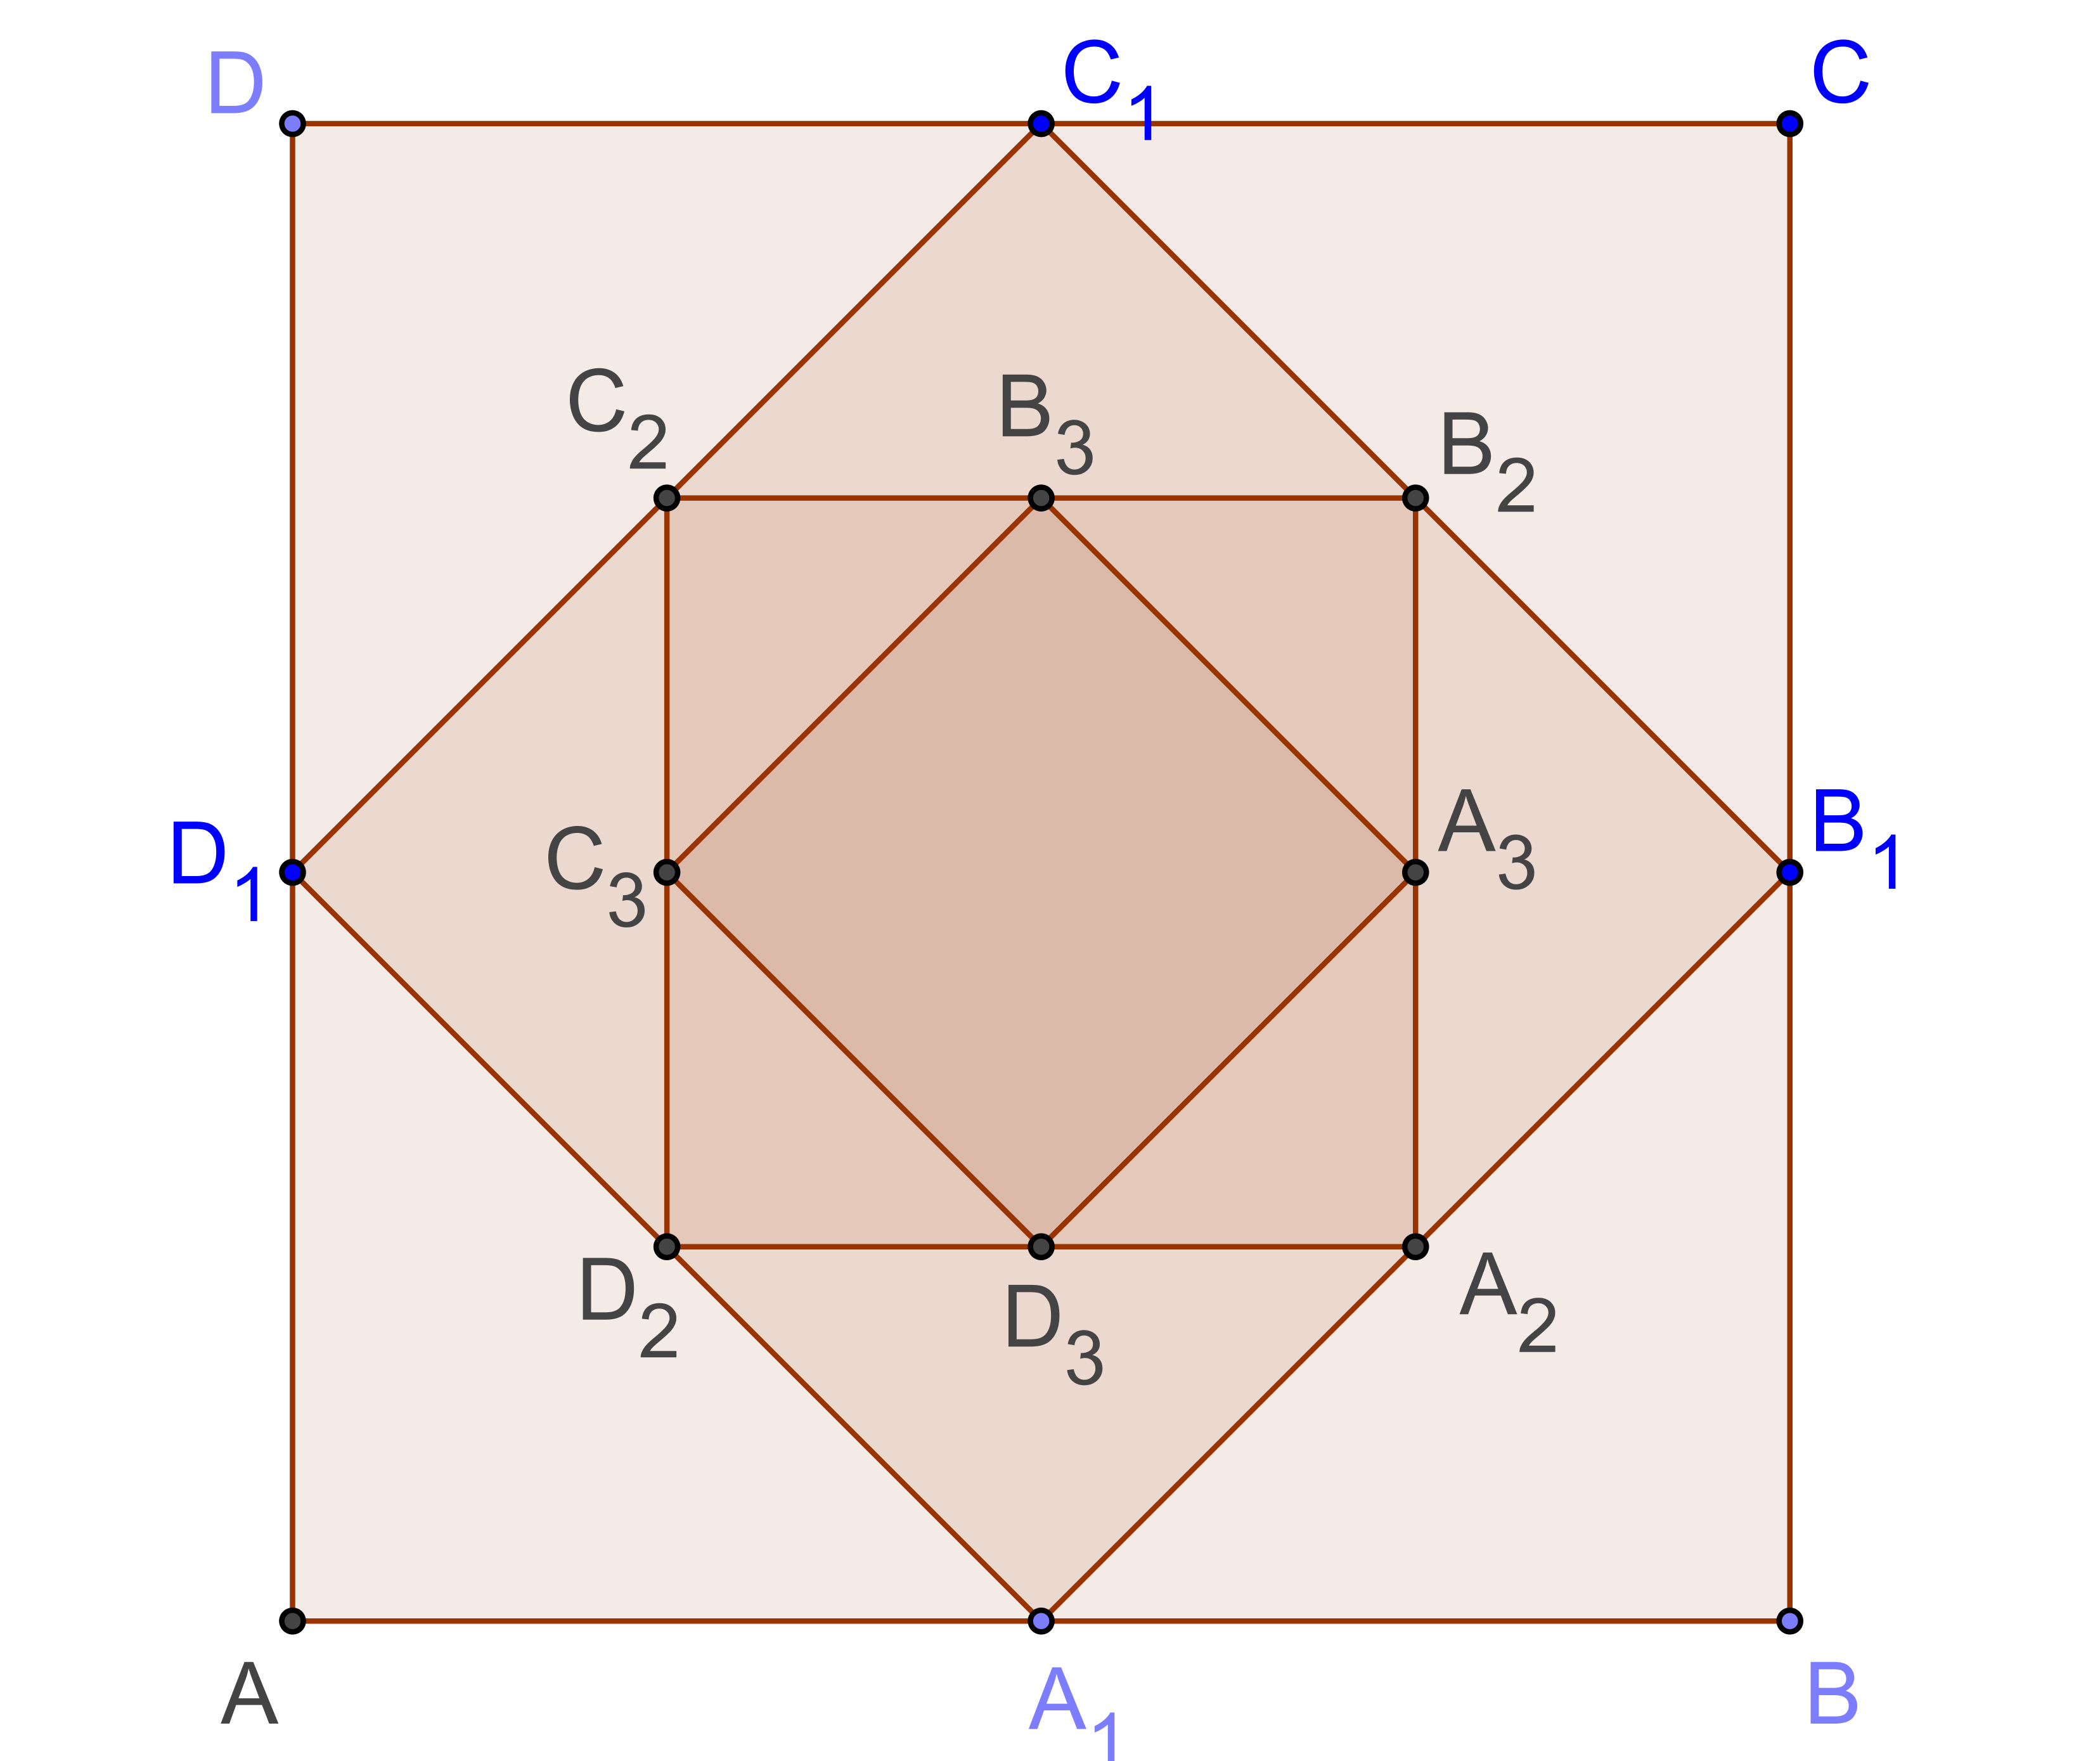
\includegraphics[width=0.5\textwidth]{30}
\end{figure}

\begin{mdframed}
\textbf{풀이 : }
\ov B{A_1}=1, \ov B{B_1}=1에서 \(\ov{A_1}{B_1}=\sqrt2\)이다.
따라서 \(S_1=(\sqrt2)^2=2\)이다.
또, \(\ov{B_1}{A_2}=\frac1{\sqrt2}\), \(\ov{B_1}{B_2}=\frac1{\sqrt2}\)에서 \(\ov{A_1}{B_1}=1\)이다.
따라서 \(S_2=1^2=1\)이다.
마찬가지로 계산하면 \(S_3=\frac12\), \(S_4=\frac14\) 등이다.
그러므로 수열 \(\{S_n\}\)은 첫항이 \(2\)이고 공비가 \(\frac12\)인 등비수열이다.
일반항을 계산하면
\[S_n=2\times\left(\frac12\right)^{n-1}=2\times2^{1-n}=2^{2-n}\]
이 된다.
따라서 
\begin{align*}
S_n 		&<0.01\\
2^{2-n}	&<\frac1{100}\\
2^{n-2}	&>100
\end{align*}
에서, \(n\)의 최솟값은 \(9\)이다.
\end{mdframed}

{\par
\raggedleft\textbf{답 : (\qquad\qquad\(n=9\)\qquad\qquad)}
\par}\bigskip\bigskip

%
\prob{}
아래 그림과 같이 한 변의 길이가 \(4\)인 정삼각형 \(ABC\)에서 \(AB\)의 중점을 \(A_1\), \(BC\)의 중점을 \(B_1\), \(CA\)의 중점을 \(C_1\)이라고 하고, 정삼각형 \(A_1B_1C_1\)의 넓이를 \(S_1\)이라고 하자.
또 \(A_1B_1\)의 중점을 \(A_2\), \(B_1C_1\)의 중점을 \(B_2\), \(C_1A_1\)의 중점을 \(C_2\)라고 하고, 정삼각형 \(A_2B_2C_2\)의 넓이를 \(S_2\)라고 하자.
이와 같은 과정을 반복하여 수열 \(\{S_n\}\)을 만들 때, \(S_5\)의 값을 구하시오.
(단, 한 변의 길이가 \(a\)인 정삼각형의 넓이는 \(\frac{\sqrt3}4a^2\)이다.)

\begin{figure}[h!]
\center
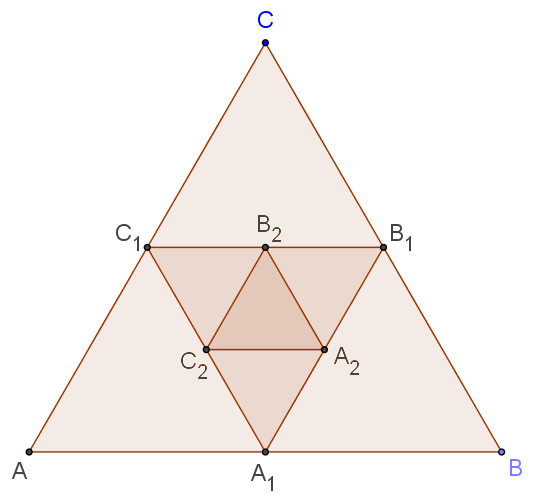
\includegraphics[width=0.5\textwidth]{31}
\end{figure}

\begin{mdframed}
\textbf{풀이 : }
\vspace{0.35\textheight}
\end{mdframed}
\ans

\clearpage

%
\exam{예금}\label{deposit_example_1}
연이율이 10\%인 은행에 100만 원을 예금한다고 하자.
1년 후에 받을 수 있는 돈은 원래 맡겨놓았던 100만 원과 이자인
\[100만 원\times\frac{10}{100}=10만 원\]
을 합친 금액인 110만 원이 된다.

%%
%\defi{이율, 원금, 이자, 원리합계}
%위의 예에서 원래 맡겨놓았던 금액인 100만 원을 \textbf{원금}이라고 하고, 늘어난 금액을 \textbf{이자}라고 한다.
%이자가 붙는 비율인 10\%는 \textbf{이율}이라고 부르며, \(r\)로 쓴다.
%위의 예에서 \(r=\frac{10}{100}=0.1\)이다.
%또한 원금과 이자를 합친 금액을 \textbf{원리합계}라고 한다.
%위의 예에서 원리합계는 110만 원이다.

%
\defi{원금, 이자, 원리합계, 이율}
은행에 돈을 맡길 때, 원래 맡겨놓은 금액을 \textbf{원금}, 늘어난 금액을 \textbf{이자}라고 한다.
원금과 이자를 합친 금액은 \textbf{원리합계}라고 부르며, 이자가 붙는 비율인 10\%는 \textbf{이율}이라고 부른다.
이율은 보통 \(r\)로 쓰며, 이율에는 연이율, 월이율 등이 있다.
위의 예에서
\begin{align*}
원금&=100만 원\\
이자&=10만 원\\
원리합계&=110만 원\\
이율&=r=\frac{10}{100}=0.1
\end{align*}

%
\exam{}\label{deposit_example_2}
예시 \ref{deposit_example_1}에서 2년 후에 받을 수 있는 돈은 얼마일까?
다음 두 가지의 방법을 생각해볼 수 있다.
\begin{enumerate}
\item
원금은 100만 원이었으니, 추가로 받을 수 있는 이자는 여전히 10만 원이다.
따라서 원리합계는 \(100+10+10=120\)만 원이다.
\item
1년 후에는 통장에 \(110\)만 원이 있으니, 추가로 받을 수 있는 이자는 \(110\times0.1=11\)만 원이 된다.
따라서 원리합계는 \(100+10+11=121\)만 원이다.
\end{enumerate}

\clearpage
%
\defi{예금, 단리, 복리}
원금을 일정한 기간동안 은행에 맡기는 것을 \textbf{예금}이라고 한다.
이때 원리합계를 구하는 방법은 두 가지로, 예시 \ref{deposit_example_2}의 (1)과 같은 방법을 \textbf{단리}, (2)와 같은 방법을 \textbf{복리}라고 한다.

\begin{figure}[h!]
\centering
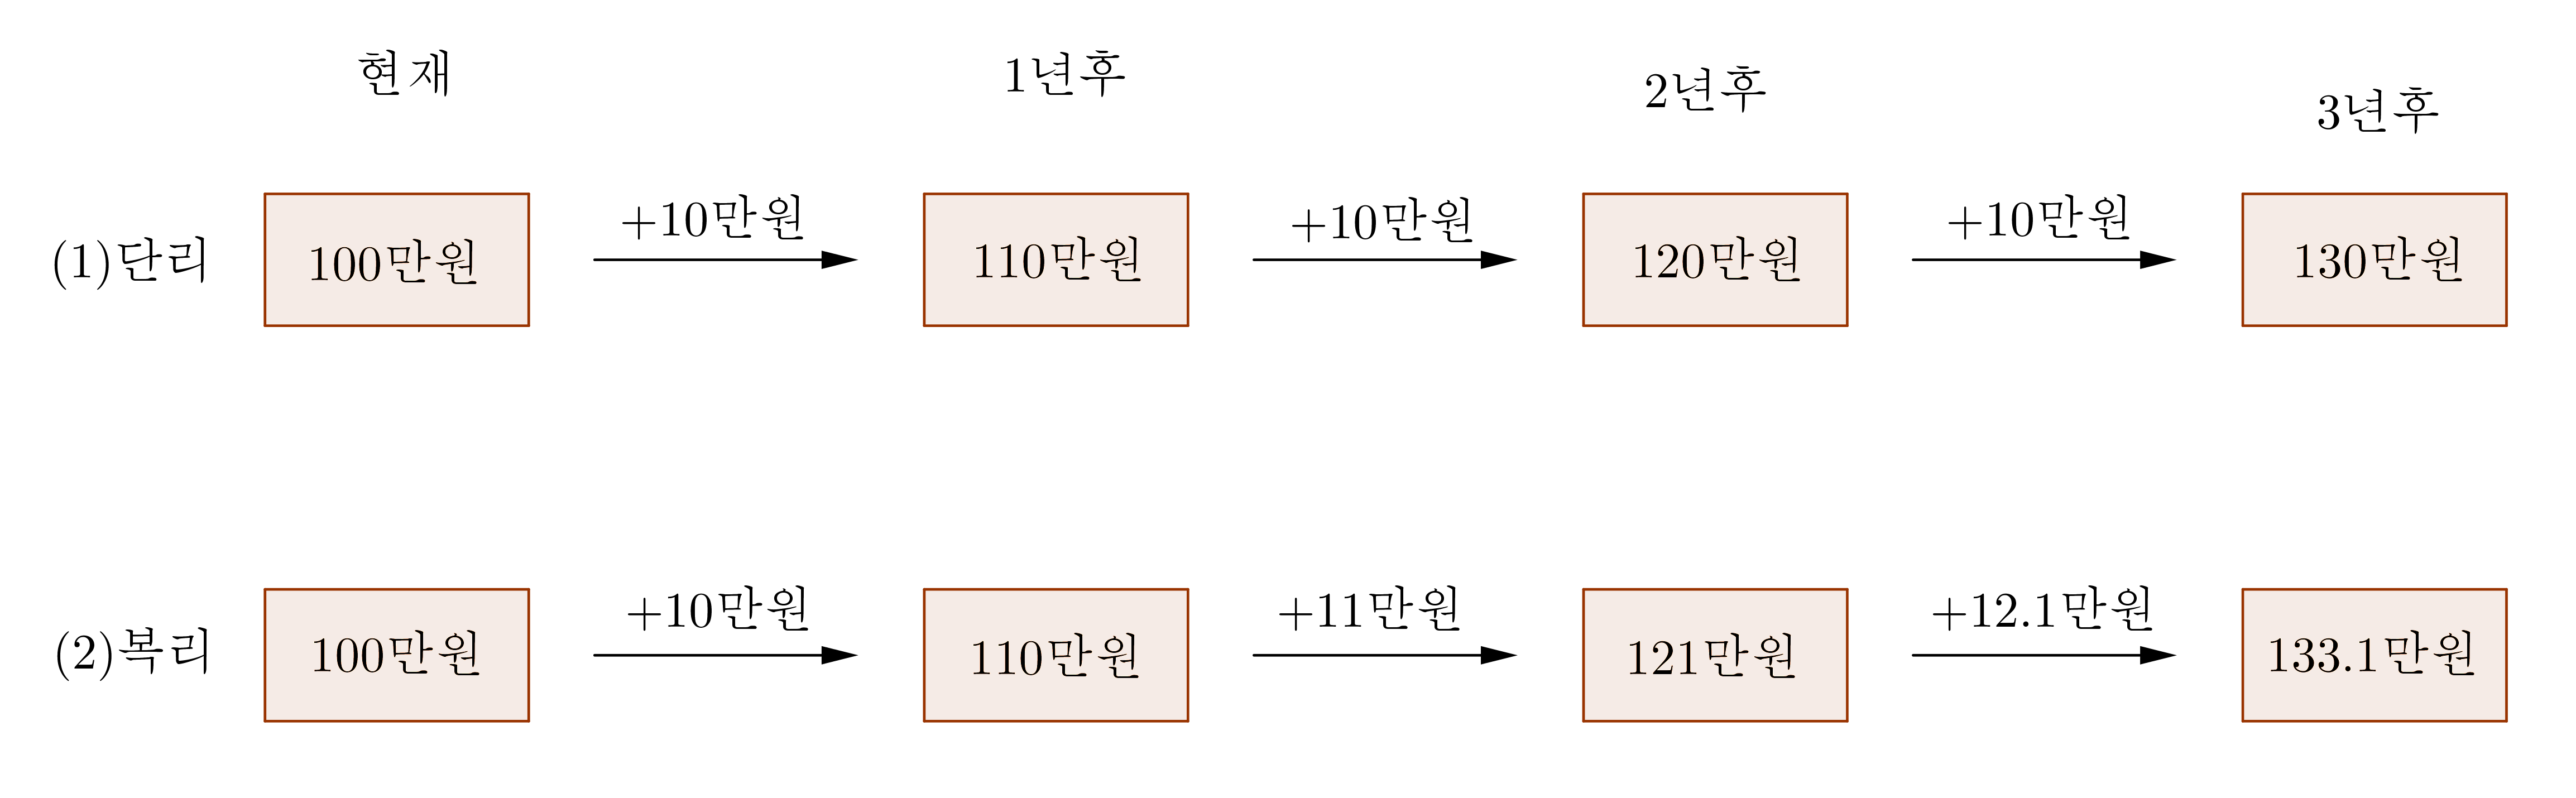
\includegraphics[width=0.8\textwidth]{34}
\end{figure}

%
\prob{}
원금 10만 원을 연이율 \(6\%\)로 예금할 때, 10년 후의 원리합계를 단리법, 복리법으로 각각 구하여라.
(단, \(1.06^{10}=1.79\)로 계산한다.)

\begin{mdframed}
\textbf{풀이 : }
\vspace{0.35\textheight}
\end{mdframed}
\ans

\clearpage
%
\exam{적금}
연이율 6\%, 매년마다 복리로 매년 초에 20000원씩 적립할 때, 10년 말의 원리합계를 구하여라.

\begin{mdframed}
\textbf{풀이 : }
10년동안 적립한 돈을 도식으로 나타내면 다음과 같다.

\begin{center}
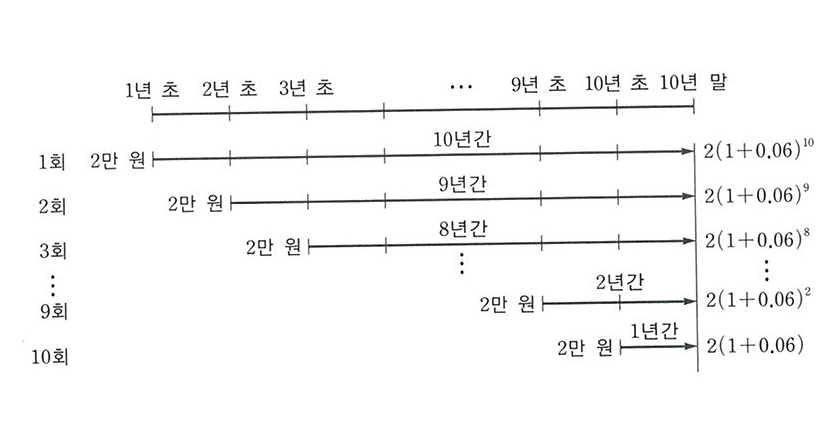
\includegraphics[width=0.7\textwidth]{deposit1}
\end{center}

원리합계를 S(만 원)이라고 하면,
\begin{align*}
S
&=2(1+0.06)+2(1+0.06)^2+2(1+0.06)^3+\cdots+2(1+0.06)^{10}\\
&=\frac{a(r^n-1)}{r-1}\\
&=\frac{2(1+0.06)(1.06^{10}-1)}{0.06}\\
&=\frac{2\times1.06\times0.8}{0.06}\\
&\approx28.26
\end{align*}
따라서, 원리합계는 28만 2600원 정도이다.
\end{mdframed}

\clearpage
%
\exam{상환}
도현이는 \(140\)만 원짜리 컴퓨터를 이달 초에 구입하고, 이달 말부터 일정한 금액씩 \(10\)개월에 걸쳐 갚으려고 한다.
월이율 \(2\)\%, 1개월마다 복리로 계산할 때, 매달 갚아야 할 금액을 구하여라.
(단, \(1.02^{10}=1.22\)로 계산한다.)

\begin{mdframed}
\textbf{풀이 : }
매달 갚는 금액을 \(a\)(만 원)이라고 가정하고, 10개월동안 적립하는 돈을 도식으로 나타내면 다음과 같다.

\begin{center}
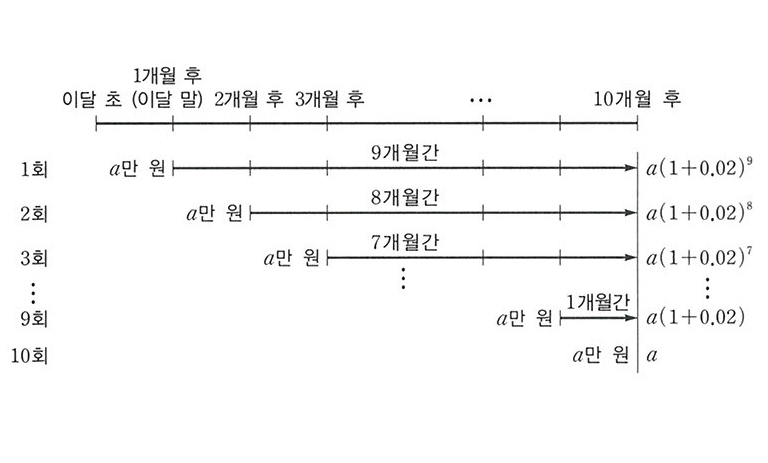
\includegraphics[width=0.7\textwidth]{deposit2}
\end{center}

원리합계를 S(만 원)이라고 하면,
\begin{align*}
S
&=a+a(1+1.02)+a(1+1.02)^2+a(1+1.02)^3+\cdots+a(1+1.02)^9\\
&=\frac{a(r^n-1)}{r-1}\\
&=\frac{a(1.02^{10}-1)}{0.02}\\
&=\frac{a\times0.22}{0.02}\\
&=11a
\end{align*}
따라서, 원리합계는 11a(만 원)이다.
이것이 140만 원과 같아야 하는데, 원리합계인 11a는 \textbf{10개월 후의 금액}이고, 140만 원은 \textbf{현재의 금액}이다.
현재의 140만 원의 가치는, 10개월 후의 140개월 후의 가치와 다르다.
만약 140만 원을 은행에 예금했다면, 10개월 후에는 \(140\times1,02^{10}=140\times 1.22=170.8\)만 원이 되어 있을 것이므로 현재의 140만 원은 10개월 후에는 170.8만 원과 같다.
따라서
\[11a=170.8\]
이 되고, \(a\approx15.53\)이다.

그러므로 매달 \(15\)만 5300원 정도를 갚으면 된다.
\end{mdframed}

\clearpage
%
\exam{연금}
올해부터 매년 말에 \(300\)만 원씩 10년 동안 받는 연금이 있다.
연이율 \(6\%\), 1년마다 복리로 계산할 때, 이 연금을 올해 초에 한꺼번에 받는다면 얼마를 받게 되는지 구하여라.
(단, \(1.06^{10}=1.79\)로 계산한다.)

\begin{mdframed}
\textbf{풀이 : }
올해 초에 한꺼번에 받는 금액을 \(S\)(만 원)이라고 하자.
이 \(S\)는 300만 원을 열 번 더한 값이지만,
\[S=300+300+300+\cdots+300\]
은 아니다. 정확히는
\[S_{올해초}=300_{올해 말}+300_{내년 말}+300_{2년 말}+\cdots+300_{10년 말}\]
이다.
도식으로 표현하면,

\begin{center}
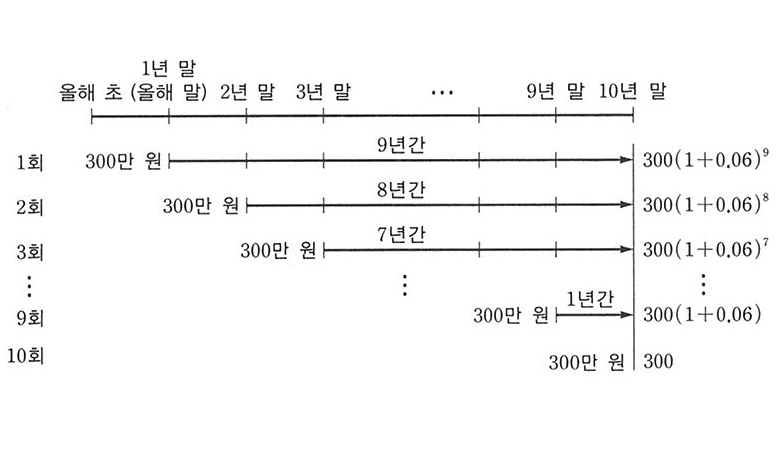
\includegraphics[width=0.7\textwidth]{deposit3}
\end{center}
이다.

따라서 10년 말을 기준으로
\[S\times1.06^{10}=300\times1.06^9+300\times1.06^8+300\times1.06+300\]
이다.
이것을 계산하면
\[1.79S=3950\]
이 되고, \(S\approx2206\)이다.

그러므로 올해 초에 한꺼번에 받는 금액은 \(2206\)만 원이다.
\end{mdframed}

%%
\section{보충·심화문제}

%
\subsection{복습}

%
\prob{}
다음을 전개하여라.
\begin{enumerate}
\item
\((x+a)^3=\)
\item
\((x-a)^3=\)
\item
\((x+a)(x+b)(x+c)=\)
\item
\((x-a)(x-b)(x-c)=\)
\item
\((a+b+c)^2=\)
\end{enumerate}

%
\prob{}
다항식 \(f(x)= ax^2+x+4\)에 대하여 \(f(x)\)를 \(x-1\), \(x-2\), \(x+3\)으로 나눈 나머지가 차례로 등차수열을 이룰 때, 상수 \(a\)의 값을 구하여라.

\begin{mdframed}
\textbf{풀이 : }
\vspace{0.35\textheight}
\end{mdframed}
\ans

\clearpage
%
\prob{삼차방정식의 근과 계수와의 관계}
삼차방정식 \(ax^3+bx^2+cx+d=0(a\neq0)\)이 세 근 \(\alpha\), \(\beta\), \(\gamma\)을 가질 때, 다음 빈칸을 채워라.
\begin{align*}
\alpha+\beta+\gamma					&=\pb{-\frac ba}\\
\alpha\beta+\beta\gamma+\gamma\alpha	&=\pb{\frac ca}\\
\alpha\beta\gamma					&=\pb{-\frac da}
\end{align*}

%
\prob{}
삼차방정식 \(x^3-3x^2+kx+4=0\)의 세 실근이 등차수열을 이룰 때, 상수 \(k\)의 값을 구하여라.

\begin{mdframed}
\textbf{풀이 : }
\vspace{0.35\textheight}
\end{mdframed}
\ans

\clearpage
%
\subsection{등비수열}

%
\prob{}
다음 등비수열 \(\{a_n\}\)에서, 공비 \(r\)을 구하고 넷째항 \(a_4\)의 값을 구하여라.
\begin{enumerate}
\item
\(1\), \(2\), \(4\), \pb{8}, \(\cdots\)
\item
\(1\), \(-2\), \(4\), \pb{-8}, \(\cdots\)
\item
\(9\), \(3\), \(1\), \pb{\frac13}, \(\cdots\)
\item
\(8\), \(-4\), \(2\), \pb{-1}, \(\cdots\)
\end{enumerate}

%
\prob{}
다음 등비수열의 일반항 \(a_n\)과 제7항을 각각 구하여라.
\begin{enumerate}
\item
\(a=2\), \(r=\frac12\)
\item
\(a=-2\), \(r=-2\)
\item
\(4\), \(8\), \(16\), \(32\), \(\cdots\)
\item
\(4\), \(2\), \(1\), \(\frac12\), \(\cdots\)
\item
\(\sqrt2\), \(-1\), \(\frac1{\sqrt2}\), \(-\frac12\), \(\cdots\)
\end{enumerate}

%
\prob{}
각 항이 실수인 등비수열 \(\{a_n\}\)의 첫째항을 \(a\), 공비를 \(r\)이라고 할 때, 다음을 구하여라.
\begin{enumerate}
\item
\(a_3=12\), \(a_6=-96\)인 등비수열의 일반항
\vspace{0.1\textheight}
\item
\(a_4=24\), \(a_8=384\)인 등비수열의 일반항
\vspace{0.1\textheight}
\item
\(a_1+a_2=5\), \(a_3+a_4=10\)인 등비수열에 대하여 \(a_5+a_6\)의 값
\vspace{0.1\textheight}
\item
\(a_3=-12\), \(a_6=96\)인 등비수열에 대하여 \(a^2+r^2\)의 값
\vspace{0.1\textheight}
\end{enumerate}

%
\prob{}
\(-4\)와 \(32\) 사이에 두 개의 수를 넣어서 전체가 등비수열을 이루도록 할 때, 이 두 수의 곱을 구하여라.
\begin{mdframed}
\textbf{풀이 : }
\vspace{0.13\textheight}
\end{mdframed}
\ans

%
\prob{}
\(3\)과 \(48\) 사이에 세 개의 양수를 넣어서 전체가 등비수열을 이루도록 할 때, 이 세 수의 곱을 구하여라.
\begin{mdframed}
\textbf{풀이 : }
\vspace{0.13\textheight}
\end{mdframed}
\ans

%
\prob{}
두 수 \(2\)와 \(162\) 사이에 세 양수 \(a\), \(b\), \(c\)를 넣어 5개의 수 \(2\), \(a\), \(b\), \(c\), \(162\)가 이 순서대로 등비수열을 이룰 때, \(a+b+c\)의 값을 구하여라.
\begin{mdframed}
\textbf{풀이 : }
\vspace{0.1\textheight}
\end{mdframed}
\ans

%
\prob{}
세 수 \(a-2\), \(a+1\), \(a-5\)가 등비수열을 이룰 때, \(a\)의 값을 구하여라.
\begin{mdframed}
\textbf{풀이 : }
\vspace{0.1\textheight}
\end{mdframed}
\ans

%
\prob{}
세 수 \(x\), \(y\), \(24\)가 이 순서대로 등차수열을 이루고, \(4\), 세 수 \(x\), \(y\)가 이 순서대로 등비수열을 이룰 때, \(x+y\)의 값을 구하여라.
(단, \(xy>0\))
\begin{mdframed}
\textbf{풀이 : }
\vspace{0.1\textheight}
\end{mdframed}
\ans

\clearpage
%
\prob{}
세 수 \(1\), \(a\), \(b\)가 이 순서대로 등차수열을 이루고, 세 수 \(a\), \(b\), \(1\)이 이 순서대로 등비수열을 이룰 때, 실수 \(a\), \(b\)의 값을 각각 구하여라.
\begin{mdframed}
\textbf{풀이 : }
\vspace{0.2\textheight}
\end{mdframed}
\ans

%
\exam{}
한 시간마다 2개로 분열하는 세포가 있다.
예를 들어, 한 개의 세포는 한 시간 후에 2개로, 두 시간 후에는 4개로, 세 시간 후에는 8개로 바뀐다.
이 세포가 7개 있을 때, 8시간 후의 세포의 개수를 구하여라.

\begin{mdframed}
\textbf{풀이 : }
\(n\)시간 후의 세포의 개수를 \(a_n\)이라고 하자.
1시간 후에 이 세포는 14개가 되므로 \(a_1=14\)이고, 2시간 후에 이 세포는 28개가 되므로 \(a_2=28\)이다.
또한 \(a_3=56\), \(a_5=112\) 이다.
이 수열 \(\{a_n\}\)은 등비수열을 이루며, \(a=14\), \(r=2\)이다.
따라서 \(a_n=14\cdot2^{n-1}=7\cdot2^n\)이고, \(a_8=7\cdot2^8=1792\)이다.
\end{mdframed}

{\par
\raggedleft\textbf{답 : (\qquad\qquad1792 개\qquad\qquad)}
\par}\bigskip\bigskip

\clearpage
%
\prob{}
두 시간마다 3개로  분열하는 세포가 있다.
예를 들어, 한 개의 세포는 두 시간 후에 3개로, 네 시간 후에는 9개로, 여섯 시간 후에는 27개로 바뀐다.
이 세포가 4개 있을 때, 6시간 후의 세포의 개수를 구하여라.
\begin{mdframed}
\textbf{풀이 : }
\vspace{0.2\textheight}
\end{mdframed}
\ans

%
\prob{}
10년마다 인구가 \(10\%\)씩 증가하는 도시가 있다.
예를 들어 현재 이 도시의 인구가 100만명이었으면, 10년 후에는 100만명의 10\%인 10만명이 증가하여 110만명이 된다.
또한 20년 후에는 110만명의 10\%인 \(110만\times\frac{10}{100}=11만명\)이 증가하여 \(110만명+11만명=121\)만명이 된다.

2016년 현재 이 도시의 인구가 200만명이었다면, 100년 후인 2116년의 이 도시의 인구는 몇 명이겠는가?
(단, 인구증가율은 일정하다고 가정하고, \(1.1^{10}=2.6\)으로 계산한다.)

\begin{mdframed}
\textbf{풀이 : }
\vspace{0.2\textheight}
\end{mdframed}
\ans
\clearpage

%
\subsection{등비수열의 합}

%
\prob{}
다음을 계산하여라.
\begin{enumerate}
\item
\(1+5+5^2+5^3+\cdots+5^n\)
\vspace{0.1\textwidth}
\item
\(3\sqrt2+6+6\sqrt2+\cdots+3\times(\sqrt2)^n\)
\vspace{0.1\textwidth}
\item
\(1+\frac12+\frac14+\frac18+\cdots+\frac1{2^n}\)
\vspace{0.1\textwidth}
\item
\(1-\frac23+\frac49-\frac8{27}+\cdots+(-\frac23)^n\)
\vspace{0.1\textwidth}
\end{enumerate}

%
\prob{}
첫째항부터 제\(4\)항까지의 합이 \(2\), 첫째항부터 제8항까지의 합이 \(8\)인 등비수열 \(\{a_n\}\)에 대하여 첫째항부터 제\(12\)항까지의 합을 구하여라.

\begin{mdframed}
\textbf{풀이 : }
\vspace{0.2\textheight}
\end{mdframed}
\ans
\clearpage

%
\prob{}
모든 항이 실수인 등비수열 \(\{a_n\}\)의 첫째항부터 제3항까지의 합이 21, 첫째항부터 제6항까지의 합이 189일 때, 첫째항부터 제8항까지의 합을 구하여라.
\begin{mdframed}
\textbf{풀이 : }
\vspace{0.2\textheight}
\end{mdframed}
\ans

%
\prob{}
공비가 실수인 등비수열 \(\{a_n\}\)에 대하여 \(a_1+a_4=3\), \(a_4+a_7=24\)가 성립한다.
이 수열의 첫째항부터 제7항까지의 합을 \(S\)라고 할 때, \(3S\)의 값은?
\begin{mdframed}
\textbf{풀이 : }
\vspace{0.2\textheight}
\end{mdframed}
\ans

\clearpage
%
\prob{}
첫째항이 \(5\), 공비가 \(2\)인 등비수열에서 첫째항부터 제\(n\)항까지의 합이 처음으로 \(500\)보다 크게 되는 자연수 \(n\)의 값을 구하여라.
\begin{mdframed}
\textbf{풀이 : }
\vspace{0.3\textheight}
\end{mdframed}
\ans

%
\prob{}
첫째항이 \(1\), 공비가 \(\frac12\)인 등비수열이 있다.
첫째항부터 제\(n\)항까지의 합을 \(S_n\)이라고 할 때, \(\left|2-S_n\right|<0.01\)을 만족하는 자연수 \(n\)의 최솟값을 구하여라.
\begin{mdframed}
\textbf{풀이 : }
\vspace{0.3\textheight}
\end{mdframed}
\ans

%%
\subsection{등비수열의 활용}

%
\prob{}
연이율 6\%의 복리로 매년 초에 30만원씩 적립하면 10년 말에는 적립 총액이 얼마나 되는지 구하여라.
(단 \(1.06^10=1.79\)로 계산한다.)
\begin{mdframed}
\textbf{풀이 : }
\vspace{0.25\textheight}
\end{mdframed}
\ans

%
\prob{}
매월 1일에 1만 원씩을 월이율 1\%의 1개월마다의 복리로 적립해나간다.
올해 1월 1일에 첫 불입금을 내었을 때, 내년 12월 31일에 받는 원리합계를 구하여라.
(단 \(1.01^10=1.28\)로 계산한다.)
\begin{mdframed}
\textbf{풀이 : }
\vspace{0.25\textheight}
\end{mdframed}
\ans

\end{document}